\documentclass[beamer]{paper}

\usepackage{quiver}
\usepackage[italic,symbolgreek]{mathastext}

% for highlighting
\usepackage{xcolor, soul}
%\makeatletter
%\let\HL\hl
%\renewcommand\hl{%
%  \let\set@color\beamerorig@set@color
%  \let\reset@color\beamerorig@reset@color
%  \HL}
%\makeatother

%\usetheme{Warsaw}
\beamertemplatenavigationsymbolsempty
%\setbeamertemplate{footline}[frame number]
%\setbeamercovered{transparent} % gray out hidden stuff
\AtBeginSection{\frame{\sectionpage}}

% Inverted colors
\definecolor{rossred}  {rgb}{1.0, 0.25,0.66}
\definecolor{rossgreen}{rgb}{0.25,0.66,0.25}
\definecolor{rossblue} {rgb}{0.25,0.66,1.0}
\renewcommand{\red}[1]{\color{rossred}  #1\color{white}}
\newcommand{\green}[1]{\color{rossgreen}#1\color{white}}
\newcommand{\blue} [1]{\color{rossblue} #1\color{white}}

\setbeamercolor{title}      {fg=white,     bg=black}
\setbeamercolor{frametitle} {fg=rossgreen, bg=black}
\setbeamercolor{normal text}{fg=white,     bg=black}
\setbeamercolor{structure}  {fg=cyan!90!black}
\setbeamercolor{block title}{fg=black,     bg=rossblue}

%%%%%%%%%%%

\newcommand{\cE}{\mathcal{E}} % bundle
\newcommand{\cH}{\mathcal{H}} % Hirzebruch surface
\newcommand{\cL}{\mathcal{L}} % line bundle

\newcommand{\Om}{\Omega}
\newcommand{\om}{\omega}

%%%%%%%%%%%

\begin{document}

% Use Computer Modern with Serif Roman Font Family
\rmfamily
\setbeamerfont{frametitle}{family=\rmfamily\selectfont}

\title[Computing Direct Sum Decompositions]
      {\textsc{Computing Direct Sum Decompositions}} % \\ over Multigraded Cox Rings

% I acknowledge that the University of Minnesota stands on Miní Sóta Makhóčhe, the homelands of the Dakhóta Oyáte.

% Abstract: It is known that the Frobenius pushforward of the structure sheaf on toric varieties splits as a sum of line bundles, and high enough pushforwards of it generate the derived category. Working over the multigraded Cox ring of a Mori Dream Space, we discuss algorithms for determining the summands of the Frobenius pushforward of the structure sheaf.

\newcommand{\lc}{\MakeLowercase}
\author[Mahrud Sayrafi]{M\lc{ahrud} S\lc{ayrafi} \\
  {\footnotesize MPI MiS}}% \\[1em]
%  {\footnotesize Joint work with Devlin Mallory \\
%    Basque Center for Applied Mathematics}}

%\institute[UMN]{U\lc{niversity} of M\lc{innesota}, T\lc{win} C\lc{ities}}

% https://www.jointmathematicsmeetings.org/meetings/national/jmm2024/2300_progfull.html
\date{{\footnotesize Effective Methods in Algebraic Geometry \\ July 30, 2024}}

\frame[plain]{\titlepage}


\begin{frame}[c,plain]
  Let's start with linear algebra. \\[1em]

  \pause
  \scalebox{0.53}{
    $
    \left(\!\begin{array}{ccccc}
         {.37}&{.28}&{.23}&{.26}&{.36}\\
         {.87}&{.76}&{.11}&{.37}&{.86}\\
         {.52}&{.82}&{.76}&{.26}&{.12}\\
         {.91}&{.91}&{.79}&{.82}&{.48}\\
         {.44}&{.13}&{.28}&{.37}&{.84}
    \end{array}\!\right) % \pause
    =
    %\underbrace{
    \left(\!\begin{array}{ccccc}
    -{.25}&{.03}+{.05}\,\mathbf{i}&{.03}-{.05}\,\mathbf{i}&{.76}&-{.04}\\
    -{.46}&{.30}-{.48}\,\mathbf{i}&{.30}+{.48}\,\mathbf{i}&-{.48}&-{.03}\\
    -{.41}&-{.57}&-{.57}&{.15}&{.44}\\
    -{.67}&-{.35}+{.3}\,\mathbf{i}&-{.35}-{.3}\,\mathbf{i}&-{.33}&-{.83}\\
    -{.32}&{.33}+{.19}\,\mathbf{i}&{.33}-{.19}\,\mathbf{i}&-{.23}&{.35}
    \end{array}\!\right)
    %}_{P}
    \cdot
    \left(\!\begin{array}{ccccc}
         {2.5}&{0}&{0}&{0}&{0}\\
         {0}&{.39}+{.47}\,\mathbf{i}&{0}&{0}&{0}\\
         {0}&{0}&{.39}-{.47}\,\mathbf{i}&{0}&{0}\\
         {0}&{0}&{0}&{.02}&{0}\\
         {0}&{0}&{0}&{0}&{.27}
    \end{array}\!\right)
    \cdot
    P^{-1}
    $
  }

  \vfill
  \pause
  \begin{enumerate}
  \item We know conditions for diagonalizability, and
  \item We have algorithms for diagonalization.
  \end{enumerate}
\end{frame}


\begin{frame}[c,plain]
  \textbf{Nonlinear Algebra:} what if we worked over a polynomial ring? \pause \vfill
  
  \scalebox{0.36}{
    \hspace*{-0.7in}
    $A = \left(\!\begin{array}{ccccccccccccccc}
    0 & 0 & 0 & 0 & 0 & x_1y_0y_1 & 0 & 0 & x_1y_0y_2 & 0 & 0 & 0 & x_0y_1y_2 & 0 & 0\\
    -x_0y_1+x_1y_1-x_1y_2 & -x_0y_2 & 0 & 0 & 0 & x_1y_2 & x_1y_2 & x_1y_2 & -x_1y_2 & -x_0y_1+x_1y_1-x_1y_2 & -x_1y_2 & 0 & x_1y_2 & x_1y_2 & x_1y_2\\
    0 & 0 & 0 & x_1y_1 & 0 & 0 & 0 & 0 & -x_1y_2 & 0 & -x_1y_2 & 0 & -x_0y_1-x_1y_2 & -x_0y_1 & -x_1y_2\\
    0 & 0 & -x_1y_2 & 0 & x_0y_0-x_1y_0-x_0y_2 & x_1y_2 & x_1y_2 & -x_1y_2 & -x_1y_2 & 0 & x_0y_2-x_1y_2 & x_0y_2 & -x_0y_2+x_1y_2 & x_0y_2+x_1y_2 & 0\\
    0 & 0 & 0 & 0 & 0 & -x_1y_2 & -x_1y_2 & x_1y_2 & x_1y_2 & x_0y_1-x_1y_1+x_1y_2 & x_1y_2 & 0 & -x_1y_2 & -x_1y_2 & -x_1y_2\\
    0 & 0 & x_1y_1 & 0 & x_1y_0 & 0 & 0 & 0 & 0 & 0 & 0 & 0 & 0 & x_0y_1 & x_1y_2\\
    0 & 0 & 0 & 0 & 0 & -x_1y_0 & 0 & -x_1y_0 & -x_1y_0 & 0 & x_0y_2 & x_0y_0 & 0 & 0 & 0\\
    x_0y_1 & x_0y_0 & 0 & 0 & 0 & 0 & 0 & x_1y_0 & 0 & 0 & 0 & 0 & 0 & 0 & 0\\
    0 & 0 & 0 & -x_1 & 0 & -x_1 & -x_1 & -x_1 & -x_1 & 0 & x_0-x_1 & x_0 & x_0 & -x_0-x_1 & 0\\
    y_1y_2 & y_0y_2 & 0 & 0 & 0 & -y_0y_1+y_1y_2 & -y_0y_1+y_1y_2 & 0 & 0 & -y_1y_2 & 0 & 0 & -y_1y_2 & y_1y_2 & 0\\
    0 & 0 & y_1y_2 & 0 & y_0y_2 & 0 & y_0y_1 & 0 & y_0y_2 & -y_1y_2 & y_0y_2 & -y_0y_2 & -y_0y_2 & -y_0y_2 & -y_0y_2\\
    -y_1 & -y_0 & 0 & 0 & 0 & 0 & 0 & 0 & y_0-y_2 & y_1 & y_0-y_2 & 0 & -y_0-y_2 & -y_0 & -y_0+y_2\\
    0 & 0 & 0 & -y_1 & 0 & -y_1 & y_1 & 0 & y_2 & 0 & 0 & 0 & y_1+y_2 & y_1 & -y_2\\
    0 & 0 & -y_1 & y_1 & -y_0 & y_1 & y_1 & 0 & y_2 & 0 & y_2 & 0 & -y_1+y_2 & y_1 & -y_2\\
    0 & 0 & 0 & 0 & 0 & -y_0+y_2 & -y_0+y_2 & y_0-y_2 & y_0-y_2 & -y_2 & -y_2 & -y_0 & y_2 & y_2 & 0\\
    0 & 0 & 0 & 0 & 0 & 0 & 0 & 0 & 0 & -y_1 & -y_0 & -y_0 & y_0 & y_0 & y_0-y_2
    \end{array}\!\right)$
  }
  \pause
  \vfill

  \scalebox{0.406}{
    \hspace*{-0.7in}
    $B = \left(\!\begin{array}{ccccccccccccccc}
    0 & 0 & 0 & 0 & 0 & 0 & 0 & 0 & 0 & 0 & 0 & 0 & 0 & 0 & 0\\
    x_1y_2 & x_0y_1-x_1y_1 & 0 & 0 & 0 & 0 & 0 & 0 & 0 & 0 & 0 & 0 & 0 & 0 & 0\\
    -y_0+y_2 & y_0-y_1 & 0 & 0 & 0 & 0 & 0 & 0 & 0 & 0 & 0 & 0 & 0 & 0 & 0\\
    0 & 0 & x_0y_1 & x_1y_1-x_1y_2 & 0 & 0 & 0 & 0 & 0 & 0 & 0 & 0 & 0 & 0 & 0\\
    0 & 0 & y_0 & y_0-y_2 & 0 & 0 & 0 & 0 & 0 & 0 & 0 & 0 & 0 & 0 & 0\\
    0 & 0 & 0 & 0 & -x_0+x_1 & x_1 & 0 & 0 & 0 & 0 & 0 & 0 & 0 & 0 & 0\\
    0 & 0 & 0 & 0 & y_0y_2-y_1y_2 & y_0y_1-y_1y_2 & 0 & 0 & 0 & 0 & 0 & 0 & 0 & 0 & 0\\
    0 & 0 & 0 & 0 & 0 & 0 & x_1y_0 & x_0y_0-x_0y_2 & 0 & 0 & 0 & 0 & 0 & 0 & 0\\
    0 & 0 & 0 & 0 & 0 & 0 & -y_1 & -y_1+y_2 & 0 & 0 & 0 & 0 & 0 & 0 & 0\\
    0 & 0 & 0 & 0 & 0 & 0 & 0 & 0 & x_0y_1-x_1y_1+x_1y_2 & x_0y_2 & 0 & 0 & 0 & 0 & 0\\
    0 & 0 & 0 & 0 & 0 & 0 & 0 & 0 & -y_1 & -y_0 & 0 & 0 & 0 & 0 & 0\\
    0 & 0 & 0 & 0 & 0 & 0 & 0 & 0 & 0 & 0 & x_1y_2 & 0 & x_0y_2 & 0 & x_0y_0-x_1y_0-x_0y_2\\
    0 & 0 & 0 & 0 & 0 & 0 & 0 & 0 & 0 & 0 & x_1y_1 & 0 & x_0y_1 & 0 & -x_1y_0\\
    0 & 0 & 0 & 0 & 0 & 0 & 0 & 0 & 0 & 0 & 0 & x_1y_0 & -x_0y_2 & x_0y_0-x_0y_2 & 0\\
    0 & 0 & 0 & 0 & 0 & 0 & 0 & 0 & 0 & 0 & y_1y_2 & y_0y_1 & 0 & y_0y_1-y_0y_2 & -y_0y_2\\
    0 & 0 & 0 & 0 & 0 & 0 & 0 & 0 & 0 & 0 & y_1 & y_1 & y_1-y_2 & y_1-y_2 & -y_0
    \end{array}\!\right)$
  }
  \pause
  \vfill

  This means $\coker A \cong \coker B$ splits as a direct sum of 7 modules.
  \pause
  \vfill

  \begin{center}
    $A$ is block \textbf{\color{rossred}diagonalizable} $\iff$ $\coker A$ \textbf{\color{rossred}splits} as a direct sum.
  \end{center}
\end{frame}


%%%%%%%%%%%%%%%%%%%%%%%%%%%%%%%%%%%%%%%%%%%%%%%%%%%%%%%%%%%%%%%%%%%%%%%%%%%%%%%%
\begin{frame} \centering \LARGE Conditions for Diagonalizability \end{frame}


{
\usebackgroundtemplate{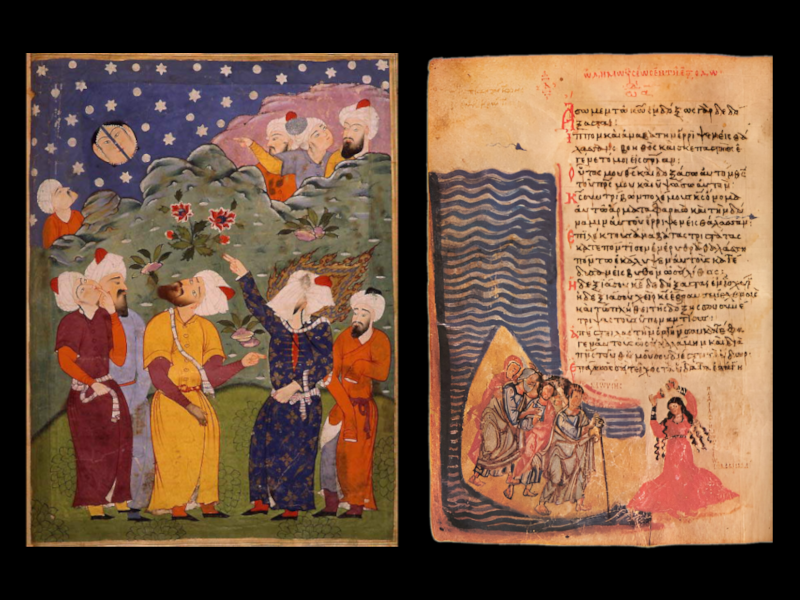
\includegraphics[height=\paperheight]{moses-mohammed.png}}
\setbeamercolor{background canvas}{bg=black}
\begin{frame}[b]
  \scriptsize{\hspace{0.35in} Falnameh, 16th century \hfill Chludov Psalter, 9th century \hspace*{0.12in}}
\end{frame}
}


\begin{frame}[t]{Warm-up: Frobenius pushforward on $\PPn$}
  % Let $\kk$ be an algebraically closed field of char $p>0$.

  Let $S = \kk[x_0,\dots,x_n]$ be a polynomial ring with $\deg x_i = 1$.

  \vfill
  \pause
  Consider the Frobenius endomorphism
  \[ F\colon S\to S \quad \text{given by} \quad x_i \to x_i^p \]

  \pause
  - Hartshorne: any $L\in\Pic\PPn$, $F_*L$ splits as a sum of line bundles. \\
  \pause
  - Rączka '24: any v.b.\ on $\PPn$, $F_*^e\cE$ splits as a sum of $\OO$'s and $\Omega$'s.
  \pause
  \begin{block}{Example: $F_*\o_{\PPn}$}
    \vspace*{-0.2in}
    \begin{align*}
      \text{When $p=3$, $n=2$:} \\
      F_*\o_{\PP2}   = \o \;\oplus\; &\o(-1)^7  \;\;\oplus\; \o(-2). \\
      \text{When $p=2$, $n=5$:} \\
      F_*\o_{\PP5}   = \o \;\oplus\; &\o(-1)^{15} \;\;\oplus\; \o(-2)^{15} \,\;\;\oplus\; \o(-3). \\
      F_*^2\o_{\PP5} = \o \;\oplus\; &\o(-1)^{120}    \;\oplus\; \o(-2)^{546}  \;\oplus\; \o(-3)^{336} \;\oplus\; \o(-4)^{21}
    \end{align*}
  \end{block}
\end{frame}


\begin{frame}[t]{Warm-up: Frobenius pushforward on toric varieties}
  Let $X$ be a smooth toric variety and consider the Cox ring
  \[ S = \bigoplus\!{}_{[D]\in\Pic{X}} \; \Gamma(X, \OO(D)) \]
  This is a \textbf{\color{rossred}polynomial ring} with a {\color{rossred}$\mathbf{\Pic{X}-}$\textbf{grading}}.

  \pause
  \begin{theorem}[Thm.~3.2, \cite{[Cox95]}]
    Every coherent sheaf on a simplicial toric variety $X$ corresponds \\
    to a finitely generated {\color{rossred}$\Pic X$-graded} $S$-module.
  \end{theorem}

  \vfill
  \pause
  - Bogvad '98, Thomsen '00: $F_*L$ totally splits for any $L\in\Pic X$. \\
  \pause
  - Achinger '13: \\ \hfill splitting of $F_*L$ characterizes smooth projective toric varieties.

  \vfill
  \pause
  \begin{block}{Example: $X = $ Hirzebruch surface of type 3, $\;F_*\o_X, \;p = 3$}
    \vspace*{-0.2in}
    \[ F_*\o_X = \o_X \;\oplus\; \o_X(-1,0)^2 \;\oplus\; \o_X(0,-1)^2 \;\oplus\; \o_X(1,-1)^3 \;\oplus\; \o_X(2,-1). \]
  \end{block}

  %% \vfill
  %% \pause
  %% \begin{block}{Remark}
  %%   The toric Frobenius is simply multiplication by $p$ on the torus.
  %% \end{block}
  %% \pause
  %% \begin{alertblock}{Funky Remark}
  %%   The $p$ need not be prime, nor even match the characteristic!
  %% \end{alertblock}
\end{frame}


%% \begin{frame}[t]{Warm-up: splitting of vector bundles on $\PPn$}
%%   Let $S = \kk[x_0,\dots,x_n]$ be a polynomial ring with $\deg x_i = 1$.

%%   \pause
%%   Let $E$ be a vector bundle of rank $r$ on $\PPn = \Proj S$.

%%   \vfill
%%   \pause
%%   \textbf{Fact:} vector bundles on $\PPn$ $\iff$ projective modules over $S$.
  
%%   \vfill
%%   \pause
%%   \begin{block}{Classical question}
%%     \centering
%%     When does $E$ \emph{split} as a direct sum of line bundles?
%%   \end{block}

%%   \vfill
%%   \pause
%%   - Grothendieck: any vector bundle on $\PP1$ splits as $E = \bigoplus\o_{\PP1}(d_i)$. \\
%%   \pause
%%   - There are indecomposable bundles of rank $n-1$ on $\PPn$, $n\!\geq\!3$. \\
%%   \pause
%%   - Horrocks--Mumford: an indecomposable rank $2$ bundle on $\PP4$ from
%%   \[ \o_{\PP4}^5 \gets \Om_{\PP4}^2(2) \oplus \Om_{\PP4}^2(2) \gets \o_{\PP4}(-1)^5. \]
%%   \pause
%%   - Hartshorne's conjecture: there are no rank 2 bundles on $\PPn, n\geq7$.

%%   %\vfill
%%   %% \pause
%%   %Notation: \\
%%   %- $\o_X$ is the structure sheaf on $X$, $\o_X(2) = \o_X(1) \otimes \o_X(1)$, etc. \\
%%   %- $\Om_X$ is the cotangent sheaf on $X$, $\Om_X^2(2) = \Om_X(1) \wedge \Om_X(1)$, etc.
%%   % TODO: add example of two resolutions on \PP1
%% \end{frame}


\begin{frame}{Warm-up: a splitting criterion for vector bundles on $\PPn$}
  \begin{theorem}[Horrocks '64]
    If for all twists $d\in\ZZ$ and $i\geq 0$, $\HH^i(\PPn, E\otimes\o_{\PPn}(d))$ is
    equal to the cohomology of a direct sum of line bundles, then $E$ splits.
  \end{theorem}

  \vfill
  \pause
  \begin{center}
    \color{rossred}``If it walks like a duck and quacks like a duck, then it's a duck.''
  \end{center}

  %\pause
  %- Computable using \emph{BGG} and \emph{Tate resolutions} over exterior algebras. \\
  %- This is a finite condition: construct the \emph{Beilinson monad} for $E$:
  %\[ B_i = \bigoplus_{j\in\ZZ} \HH^{j-i}\left(\PPn, E\otimes\o_{\PPn}(-j)\right) \otimes \Om_{\PPn}^j(j). \]

  \vfill
  \pause
  - Dolgachev '82: Weighted projective spaces \\
  - Ottaviani '89: $\mathrm{Gr}(k,n)$ and quadric hypersurfaces in $\PPn, n\geq4$ \\
  - Fulger--Marchitan '11: rank 2 bundles on Hirzebruch surfaces \\
  %- Products of projective spaces: Eisenbud--Erman--Schreyer ('15)

  \vfill
  \pause
  \begin{block}{First Goal}
    \centering
    Prove a similar splitting criterion over normal toric varieties, \pause \\
    i.e., a condition for diagonalizability of graded matrices.
  \end{block}
\end{frame}


%% \begin{frame}[t]{Warm-up: Frobenius pushforward on toric varieties}
%%   Let $X$ be a smooth toric variety and consider the Cox ring
%%   \[ S = \bigoplus\!{}_{[D]\in\Pic{X}} \; \Gamma(X, \OO(D)) \]

%%   \pause
%%   \begin{theorem}[Thm.~3.2, \cite{[Cox95]}]
%%     Every coherent sheaf on a simplicial toric variety $X$ corresponds \\
%%     to a finitely generated $\Pic X$-graded $S$-module.
%%   \end{theorem}

%%   \vfill
%%   \pause
%%   Fact: for any toric variety, $S$ is a \textbf{multigraded} polynomial ring.
%%   \pause
%%   Upshot: commutative algebra over a toric variety is easy! \\
%%   \pause
%%   \hfill i.e. we have monomial orderings, Gr\"obner bases, syzygies, etc.
%% \end{frame}


\begin{frame}[t]{What makes a splitting criterion strong?}
  When $X = \PP{n_1}\times\PP{n_2}\times\cdots\times\PP{n_t}$:
  \begin{theorem}[Eisenbud--Erman--Schreyer '15]
    Let $E$ be a vector bundle on $X$ whose sheaf cohomology matches that of
    \( \sum_{i=1}^r \OO(\underline{d}_i)^{e_i}, \) for $\underline{d}_i\in\ZZ^r$.
    {\color{rossred}If $\underline{d}_r \le \cdots \le \underline{d}_1$}, then $E$ splits.
  \end{theorem}
  \pause
  - Holds in arbitrary dimension and Picard rank. \\
  - But {\color{rossred}only when $\Nef X = \Eff X = $ the positive orthant}.

  \vfill
  \pause
  When $X = \PP{}(\o\oplus\o(a_1)\oplus\cdots\oplus\o(a_s)) \to \PP{t}$:
  \pause
  \begin{theorem}[Brown--S. '22]
    Let $E$ be a vector bundle on $X$ whose sheaf cohomology matches that of
    \( \sum_{i=1}^r \OO(b_i, c_i)^{e_i}. \)
    {\color{rossred}If $(b_r, c_r) \le \cdots \le(b_1, c_1)$}, then $E$ splits.
  \end{theorem}
  \pause
  - Holds in arbitrary dimension, but {\color{rossred}only Picard rank = 2}. \\
  - Now $\Nef X = $ the positive quadrant, but {\color{rossgreen}$\Eff X$ can be larger}.
\end{frame}


\begin{frame}[t]{Ingredient list for other toric varieties}
  When $X$ is an arbitrary smooth projective toric variety:
  \begin{theorem}[S. '24]
    Let $E$ be a vector bundle on $X$ whose sheaf cohomology matches that of
    \( \sum_{1}^r \OO(D_i)^{e_i}\!, \) $D_i\in\Pic X$\!.
    {\color{rossred}If $D_{i+1}\!-\!D_i$ is ample}, then $E$ splits.
  \end{theorem}
  \pause
  - Holds in {\color{rossgreen}arbitrary} dimension and Picard rank. \\
  - Holds for {\color{rossgreen}arbitrary} $\Nef X$ and $\Eff X$. \\ \pause
  - But: the additional hypothesis on $E$ is stronger \pause ... probably!

  \vfill
  \pause
  \textbf{\color{rossred} Upshot:} if $\coker A$ satisfies the conditions above, $A$ diagonalizes.

  \vfill
  \pause
  \begin{exampleblock}{}
    \textbf{Key ingredient:} \\
    \centering
    a resolution of the diagonal for $X$, with special properties %such that we can prove \\
    % \hl{for all $D$ ample, if $E = \o(-D)$ the ``page'' is ``upper triangular''.}
  \end{exampleblock}
  
  \pause
  \textbf{Candidate:} Hanlon--Hicks--Lazarev's resolution of the diagonal.%\\ \pause
  % \textbf{New tool:} vanishing theorems on line bundles and $\QQ$-divisors.
\end{frame}


%%%%%%%%%%%%%%%%%%%%%%%%%%%%%%%%%%%%%%%%%%%%%%%%%%%%%%%%%%%%%%%%%%%%%%%%%%%%%%%%
\begin{frame}
  \centering
  \LARGE Algorithm for Diagonalizability \\[1em]
  \footnotesize Joint work with Devlin Mallory \\
  Basque Center for Applied Mathematics
\end{frame}


{
\usebackgroundtemplate{
\includegraphics[height=\paperheight]{odysseymonkey}}
\setbeamercolor{background canvas}{bg=black}
\begin{frame}
\end{frame}
}


\begin{frame}{Frobenius pushforward on Grassmannians}
  We can still consider the Cox ring
  \[ S = \bigoplus\!{}_{[D]\in\Pic{X}} \; \Gamma(X, \OO(D)) \]
  For Grassmannians this coincides with the coordinate ring.

  \pause
  \begin{block}{Example: $X = \mathrm{Gr(1,3)}, \;F_*\o_X, \;\char \kk = p = 3$}
    Working over the ring:
    \[ S = \frac{\kk[P_{01},P_{02},P_{12},P_{03},P_{13},P_{23}]}{P_{12}P_{03}-P_{02}P_{13}+P_{01}P_{23}} \]
    When $p = 3$:
    \[ F_*\o_X = \o \oplus \o(-1)^{44} \oplus \o(-2)^{20} \oplus A^4 \oplus B^4, \]
    where $A$ and $B$ are rank 2 indecomposable bundles. \\
    \hfill (c.f. [Raedschelders--Špenko--Van den Bergh, '17])
  \end{block}
\end{frame}


\begin{frame}{Frobenius pushforward on Mori Dream Spaces}
  This is the natural setting to work over the Cox ring
  \[ S = \bigoplus\!{}_{[D]\in\Pic{X}} \; \Gamma(X, \OO(D)). \]
  Hu--Keel: $X$ is an $MDS$ $\iff$ the Cox ring is finitely generated.

  \vfill
  \pause
  \begin{exampleblock}{Examples}
  \; - Projective toric varieties \\
  \; - Grassmannians and flag varieties \\
  \; - Determinantal varieties \\
  \; - Many complete intersection rings \\
  \; - Smooth Fano varieties over $\CC$ \\
  \; - $\overline{M}_{0,n}$ for $n\leq 6$ (7,8,9 are unknown)
  \end{exampleblock}
\end{frame}


\begin{frame}{Frobenius pushforward on Mori Dream Spaces}
  \begin{block}{Example: $X = \mathrm{Bl}_4\PP2, \; F_*^2\o_X, \; \char \kk = p = 2$}
    Working over the $\ZZ^5$-graded Cox ring\vspace*{-0.15in}
    \[ S = \kk[x_1,\dots,x_{10}]/\text{(five quadric Pl\"ucker relations)} \]
    \pause
    With degrees \vspace*{-0.15in}
    \[
    \left(\!\begin{array}{cccccccccc}
      0&0&0&0&1&1&1&1&1&1 \\
      1&0&0&0&-1&-1&-1&0&0&0 \\
      0&1&0&0&-1&0&0&-1&-1&0 \\
      0&0&1&0&0&-1&0&-1&0&-1 \\
      0&0&0&1&0&0&-1&0&-1&-1
    \end{array}\!\right)
    \]
    In the basis:
    \[ \Pic X \cong \langle H \rangle \oplus \langle E_1 \rangle \oplus \langle E_2 \rangle \oplus \langle E_3 \rangle \oplus \langle E_4 \rangle. \]
  \end{block}
\end{frame}


\begin{frame}{Frobenius pushforward on Mori Dream Spaces}
  \begin{block}{Example: $X = \mathrm{Bl}_4\PP2, \; F_*^2\o_X, \; \char \kk = p = 2$}
    \vspace*{-0.15in}
    \begin{align*}
      F_*^2\o_X = {\o_{X}^{1}}
      &\oplus {\o_{X}^{2}\ \left(-1,\,1,\,0,\,0,\,0\right)} \oplus {\o_{X}^{2}\ \left(-1,\,0,\,1,\,0,\,0\right)} \\ 
      &\oplus {\o_{X}^{2}\ \left(-1,\,0,\,0,\,1,\,0\right)} \oplus {\o_{X}^{2}\ \left(-1,\,0,\,0,\,0,\,1\right)} \\
      &\oplus {\o_{X}^{2}\ \left(-2,\,1,\,1,\,1,\,1\right)} \oplus B \oplus G,
    \end{align*}
    where $B, G$ are rank 3 and rank 2 indecomposables. \\
    \hfill (c.f. [Hara, '15])
  \end{block}
\end{frame}


{
\usebackgroundtemplate{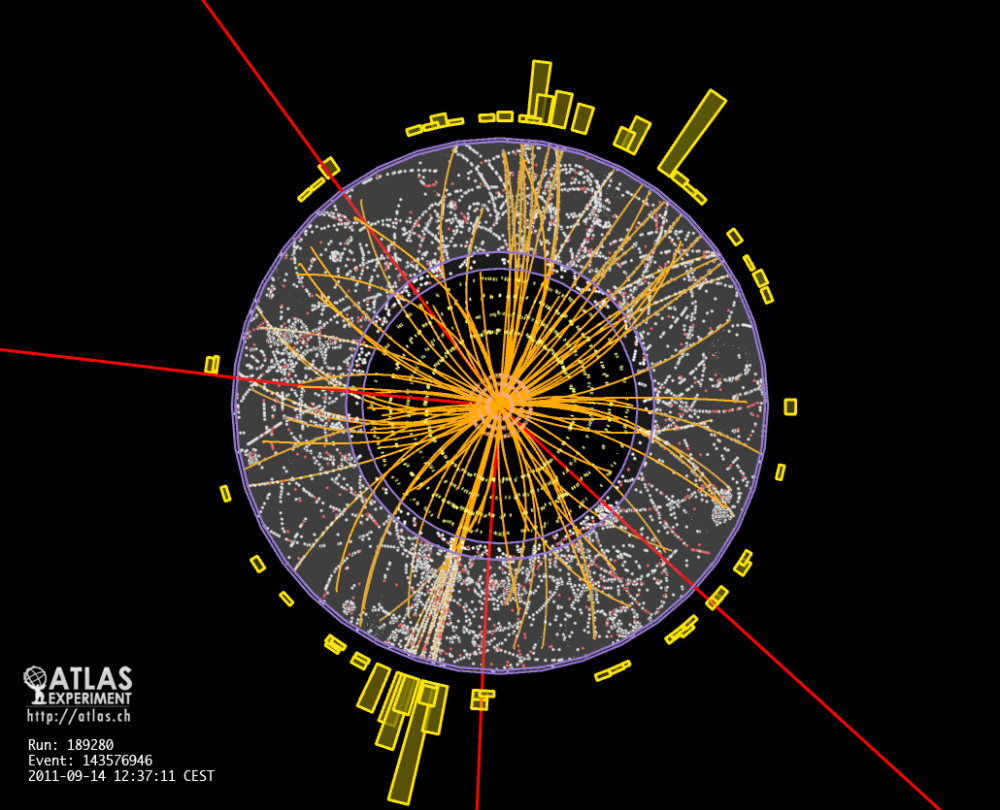
\includegraphics[width=\paperwidth]{higgs}}
\setbeamercolor{background canvas}{bg=black}
\begin{frame}
\end{frame}
}


\begin{frame}{The splitting algorithm}
  \begin{alertblock}{The ``Meataxe'' algorithm for graded $S$-modules:}
    Input: finitely generated graded module $M$ over an algebra.
    \pause
    \begin{enumerate}
    \item Compute $\Hom(M, M)_0$ \\ \pause
      Note: the degree zero part only, so \textbf{\color{rossgreen}multigrading helps!} \pause
    \item Find element $h$ corresponding to an idempotent \\ \pause
      \begin{itemize}
      \item Often a generator of $\Hom$ is already an idempotents! \pause
      \item In characteristic $p > 0$, we find a general endomorphism $A$
        and prove that $(A-\lambda I)^\ell$ is idempotent for $\ell = kp(p^e-1)$. \pause
      \end{itemize}
    \item Find the image and cokernel of $h$;
    \item Repeat.
    \end{enumerate}
  \end{alertblock}

  %% \vfill
  %% \pause
  %% \begin{lemma}
  %%   Let $M$ be an $R$-module, and let $A\in\End_R(M)$. If the induced action of $A$ on $M/mM$ is idempotent, then $M$ admits a direct sum decomposition $N\oplus M/N$, where $N\cong \im A$.
  %%   % Let $A$ be an endomorphism of a $k$-vector space such that all eigenvalues of $A$ are contained in $k$. If $\lambda$ is an eigenvalue of $A$, then some power of $A-\lambda I$ is an idempotent.
  %% \end{lemma}
\end{frame}


\begin{frame}{Other Applications}
  Even in absence of a multigrading, explicit computations of direct
  sum decompositions is useful for mathematical experiments: \\[1em]
  \; - Finite Cohen--Macaulay-type property of singularities; \\
  \; - $F$-representation type property of cubic surfaces; \\
  \; - Structure of syzygies over Artinian rings. \\

  \vfill
  \pause
  \begin{block}{Question for the road:}
    \centering
    What are applications of diagonalization of polynomial \\
    matrices in algebraic geometry and nonlinear algebra?
  \end{block}
\end{frame}


%% \begin{frame}[t]{Frobenius pushforward on determinantal varieties}
%%   \textbf{Fact:} a determinantal variety $X$ is a Mori dream space. \\
%%   \hfill (i.e. the Cox ring is a finitely generated algebra.)

%%   \vfill
%%   Singh: does $F^e_*\OO_X$ have finitely many classes of summands? \\
%%   This is known as having \emph{globally finite $F$-representation type}.

%%   \begin{block}{Problem}
%%     Classify MDS with globally finite $F$-representation type.
%%   \end{block}

%%   \begin{alertblock}{Upshot}
%%     Determining line bundle summands is easy over the Cox ring.
%%   \end{alertblock}

%%   \vfill
%% \end{frame}


\begin{frame}[t]{References}
  \scriptsize{
    - Hartshorne '70, \hfill\textit{Ample subvarieties of algebraic varieties} \\[1.5em]
    - Bogvad '98, \hfill\textit{Splitting of the direct image of sheaves under the Frobenius} \\[1.5em]
    - Thomsen '00, \hfill\textit{Frobenius direct images of line bundles on toric varieties} \\[1.5em]
    - Achinger '13, \hfill\textit{A characterization of toric varieties in characteristic $p$} \\[1.5em]
    - Hara '15, \hfill\textit{Looking out for Frobenius summands on a blown-up surface of $\PP2$} \\[1.5em]
    - Raedschelders, Špenko, Van den Bergh '17, \\ \hfill\textit{The Frobenius morphism in invariant theory} \\[0.5em]
    - Rączka '24, \hfill\textit{Frobenius pushforwards of vector bundles on projective spaces}
  }

  \renewcommand{\section}{\subsection}
  \printbibliography
\end{frame}

\end{document}

% Local Variables:
% tab-width: 2
% eval: (visual-line-mode)
% End:
